\documentclass[11pt, a4paper]{article}
\usepackage{lipsum}
\usepackage{helvet}
\usepackage{anyfontsize}
\usepackage[dvipsnames]{xcolor}
\usepackage{graphicx} 
\usepackage{tabularx}
\usepackage{enumitem}
\usepackage{fancyhdr}
\usepackage[ddmmyy]{datetime}
\usepackage{geometry}
\usepackage{cite}
\usepackage[ngerman]{babel}
\usepackage{bibgerm}
\usepackage{ragged2e}
\usepackage{hyperref}
\usepackage[german]{cleveref}


%%%%%%%%%%%%%%%%%%%% PRÄAMBEL %%%%%%%%%%%%%%%%%%%% 
%Dates
\renewcommand{\familydefault}{\sfdefault}
\renewcommand{\dateseparator}{.}
\setlength{\parindent}{1.5em}
\setlength{\parskip}{0.5em}

%Papersize
\geometry{a4paper, includehead, includefoot, top=2.5cm, bottom=2cm, left=2.5cm, right=2.5cm} 

%Tablestuff
\def\arraystretch{1.5}
\newcolumntype{L}{>{\RaggedRight} X}

%Headers
\pagestyle{fancy}
\renewcommand{\headrulewidth}{0pt}
\renewcommand{\footrulewidth}{0pt}
\setlength{\headheight}{26pt}
\lhead{
	\raisebox{-.2\height}{
		
\includegraphics{doc_images/EB.png}}
	\textcolor{gray}{\LARGE\ \&}
	\raisebox{-.3\height}{
		
\includegraphics[scale=0.6]{doc_images/LL.png}}
	\hspace{.3cm}
	\textbf{\color{SpringGreen}2019S}
}
\rhead{\scalebox{.7}[1.0]{\large\textbf{Informatikdidaktik \& transferable skills}}}
\fancyfoot[L]{\footnotesize \bottomleftfooter}
\fancyfoot[C]{\footnotesize \today\ // \currenttime}
\fancyfoot[R]{\footnotesize \thepage}
%%%%%%%%%%%%%%%%%%%% PRÄAMBEL %%%%%%%%%%%%%%%%%%%% 

%%%%%%%%%%%%%%%%%%%% INFOS %%%%%%%%%%%%%%%%%%%% 
\newcommand{\authortext}{Hurbean Alexander \& Ploder Bernhard}
\newcommand{\situation}{Prüfungsangst (im Studium)}

\newcommand{\bottomleftfooter}{Situation 1 - ebll19s - de}
%%%%%%%%%%%%%%%%%%%% INFOS %%%%%%%%%%%%%%%%%%%% 

\begin{document}
\begin{tabular}{l l} 
Authors: & \textbf{\textcolor{blue}{\large\authortext}}\\ 
Situation: & \textbf{\textcolor{blue}{\large\situation}}
\end{tabular}

\vspace{1em}

\centerline{
	\fcolorbox{white}{SpringGreen}{
		\fontsize{21}{12} \selectfont 
			Description of Situation / Triggers / Effects (table)}}

\vspace{1em}

\begin{table}[h!]
	\begin{tabularx}{\textwidth}{|p{0.3cm}|p{3.5cm}|L|}
		\hline
		1 & Spielfeld-Nummer                       & 35 – 39 Universität \\
		\hline
		2 & Ausgangspunkt                          & 
		Du hast eine wichtige Prüfung schon zum zweiten Mal nicht geschafft.
		Nun bleiben dir nur noch 3 weitere Versuche, zwei davon sind kommissionell. \\
		\hline
		3 & Wirkungen                              &
		Deine Reaktion darauf ist abhängig von deiner Persönlichkeit und vergangenen Erfahrungen:
		\begin{itemize}[noitemsep, topsep=0pt]
			\item {[1,2,3]} Du fühlst dich durch die wiederholten Rückschläge entmutigt und findest es immer schwerer dich mit dem Thema auseinanderzusetzen. Dies wirkt sich auch auf andere Arbeitsbereiche negativ aus. Du hast erhöhte Prüfungsangst und glaubst, dass dein Erfolg sehr unwahrscheinlich ist. \texttt{(-3 Motivationspunkt)}
			\item {[4,5]} Auf vergangene Ergebnisse legst du nicht viel Wert und du lernst für die nächste Prüfung so, iwe für die ersten beiden Antritte. Durch Stress (hohe Kursbelastung) und ineffizientes lernen verbessert sich deine Situation jedoch nicht. \texttt{(-1 Motivationspunkte)}
			\item {[6]} Trotz Rückschlage bist du entschlossen und beschließt dich für den nächsten Prüfungsantritt möglichst gut vorzubereiten um deine Erfolgschancen zu maximieren, indem du mehr Zeit investierst und z.B. eine Nachhilfe aufsuchst. \texttt{(+1 Motivationspunkt)}
		\end{itemize} \\
		\hline
		4 & Differenzierung \newline (falls nötig) & 
		\begin{itemize}[noitemsep, topsep=0pt]
			\item Persönlichkeit: \texttt{[Pessimist, Optimist]}
			\item Soziales Umfeld: \texttt{[Eltern, Freunde]}
			\item Finanzielle Mittel: \texttt{[(kein) Geld für Nachhilfe etc.]}
		\end{itemize} \\
		\hline
		5 & Auslöser                               & 
		\begin{itemize}[noitemsep, topsep=0pt]
			\item Negative/Positive vergangene Erfahrungen mit dem Prüfungsfach
			\item Sozialer Druck durch Kollegen/Freunden/Familie
			\item Andere Prüfungen die nicht erfolgreich waren
			\item Generelles Interesse/Desinteresse an dem Fach
		\end{itemize} \\
		\hline
	\end{tabularx}
\end{table}
\newpage

\section*{Theoretische Begründung der behaupteten Wirkung/en}
Es gibt viele Menschen, die die Spannungssituation einer Prüfung nicht als leistungsfördernden Antrieb einsetzten können sondern durch Angst und dysfunktionale Vorbereitung nicht ihr volles Potential ausschöpfen können oder sogar gänzlich blockiert werden. \cite{Holm-Hadulla2009}

"Leichte Arbeitsstörungen, Selbstzweifel und ein gewisses Maß an Angst gehören sowohl zur Arbeit als auch zu Prüfungen und sind daher als normal anzusehen." \cite{Holm-Hadulla2009}

Ab wann jedoch diese leichten Ängste und Arbeitshindernisse zu einem ernsthaften Problem werden und das Arbeiten bzw. Lernen übermäßig stark beeinflussen kann von Person zu Person unterschiedlich sein. Manche Menschen können sich vielleicht auch in stressigen und unvorteilhaften Situationen noch auf das Wesentliche konzentrieren und verlieren möglicherweise nur wenig Arbeitsleistung. Wo hingegen es andere Menschen gibt die bereits komplett überfordert sind sobald etwas nicht nach Plan läuft oder sie mit unvorhergesehene Rückschläge umgehen müssen.

Prüfungsängste, und die daraus resultierenden Arbeitsstörungen, können in manchen\\ Fällen so schlimm werden, dass die Folgen Kriterien für eine psychische Störung erfüllen. Sie könnten aber auch Begleiterscheinungen von bereits vorhandenen psychischen Störungen sein. \cite{Holm-Hadulla2009}

Oftmals sind Probleme wie unzureichender Schlaf bzw. Ruhe, nicht ausreichend physische Aktivität, schlechte Ernährung aber auch kein oder mangelndes Zeitmanagement Faktoren die ganz erheblich dazu betragen, dass Prüfungsangst überhaupt entsteht. Häufig führen auch negatives und irrationales Denken über Prüfungen und Noten, aber auch das Gefühl, keine Kontrolle über die Prüfungssituation ansich zu haben zu Prüfungsängsten. \cite{hashmat2008factors}

Es wird angenommen, dass Prüfungsängste die nicht richtig behandelt werden und über längere Zeiträume bestehen Schüler bzw. Studenten immer mehr negativ beeinflussen. 

Wie bereits erwähnt ist Prüfungsangst ein vielschichtiges Phänomen welches vor allem Sorgen, die Gefühlswelt und das Verhalten gegenüber möglichen negativen Resultaten der akademischen Laufbahn involviert. (Chapell et al. 2005; Mulkey \& O’ Neil, 1999, zitiert nach \cite{barrows2013anxiety})

Ein weiterer Punkt der ebenfalls zu beachten ist, ist die Selbstwirksamkeitserwartung aber auch das Selbstwertgefühl einer Person. Selbstwirksamkeitserwartung ist die Erwartung einer Person ein gewünschtes Ziel zu erreichen, aufgrund der eigenen Kompetenzen.

So kann, in bestimmten Fällen, die Selbstwirksamkeitserwartung eines Menschen die Effekte und Auswirkungen von Prüfungsängsten variieren bzw. in gewissem Maße kontrollieren. \cite{barrows2013anxiety}

\newpage
\section*{Empirische Belege für das Eintreten der behaupteten Wirkungen/en}

	Die herangezogenen Papers stellen verschiedene Zusammenhänge für Ursache von \\Prüfungsangst, beziehungsweise Einflussfaktoren, dar. Es werden sowohl Ursache als auch gegenwirkende Faktoren betrachtet, wie Selbstwirksamkeitserwartung, die gegen \\Prüfungsangst hilft, oder diese zumindest mildert.

	Im Journal of Pakistan Medical Association, wurde ein Artikel veröffentlicht, der über verschiedene Einflussfaktoren berichtet, die bei Medizinstudenten Prüfungsangst verursachen. Über vier Wochen hinweg wurden Fragebögen mit Visuellen Analogskalen genutzt, mit 17 Fragen zu Lebensstil, Studium, psychologischen Problemen und zum Benotungssytem. Die Skalen selbst wurden genutzt um Prüfungsangst zu messen (siehe \cref{fig:vas}) \cite{hashmat2008factors}

	\begin{figure}[p]
		\centering
		
\includegraphics{img/VAS.png}
		\caption{Eine Visuelle Analogskala die genutzt wird, um Schmerzen zu messen \cite{hashmat2008factors}}
		\label{fig:vas}
	\end{figure}

	Von den 200 Fragebögen sind 120 zurück gekommen, die dann mit SPSS ausgewertet wurden. Der durchschnittliche Wert für Prüfungsangst war 64. Die Skala war in drei Teile geteilt, 0-30 (wenig Prüfungsangst), 40-60 (mäßige Prüfungsangst), 70-100 (starke Prüfungsangst). Männliche Studenten hatten durchschnittlich 34 und weibliche 72 angekreuzt. Die Verteilung der Geschlechter unter den Studenten war 25.8/74.2 (männlich/weiblich). Es wurden pro Geschlecht die Faktoren ermittelt (siehe \cref{fig:jpmatable}). Es wird gezeigt, dass unter weiblichen Studenten die hohe Prüfungsangst einen hohen Zusammenhang mit zu starken Kursbelastungen und auch zu wenig sportlichen Aktivitäten bildet. \cite{hashmat2008factors}

	\begin{figure}[p]
		\centering
		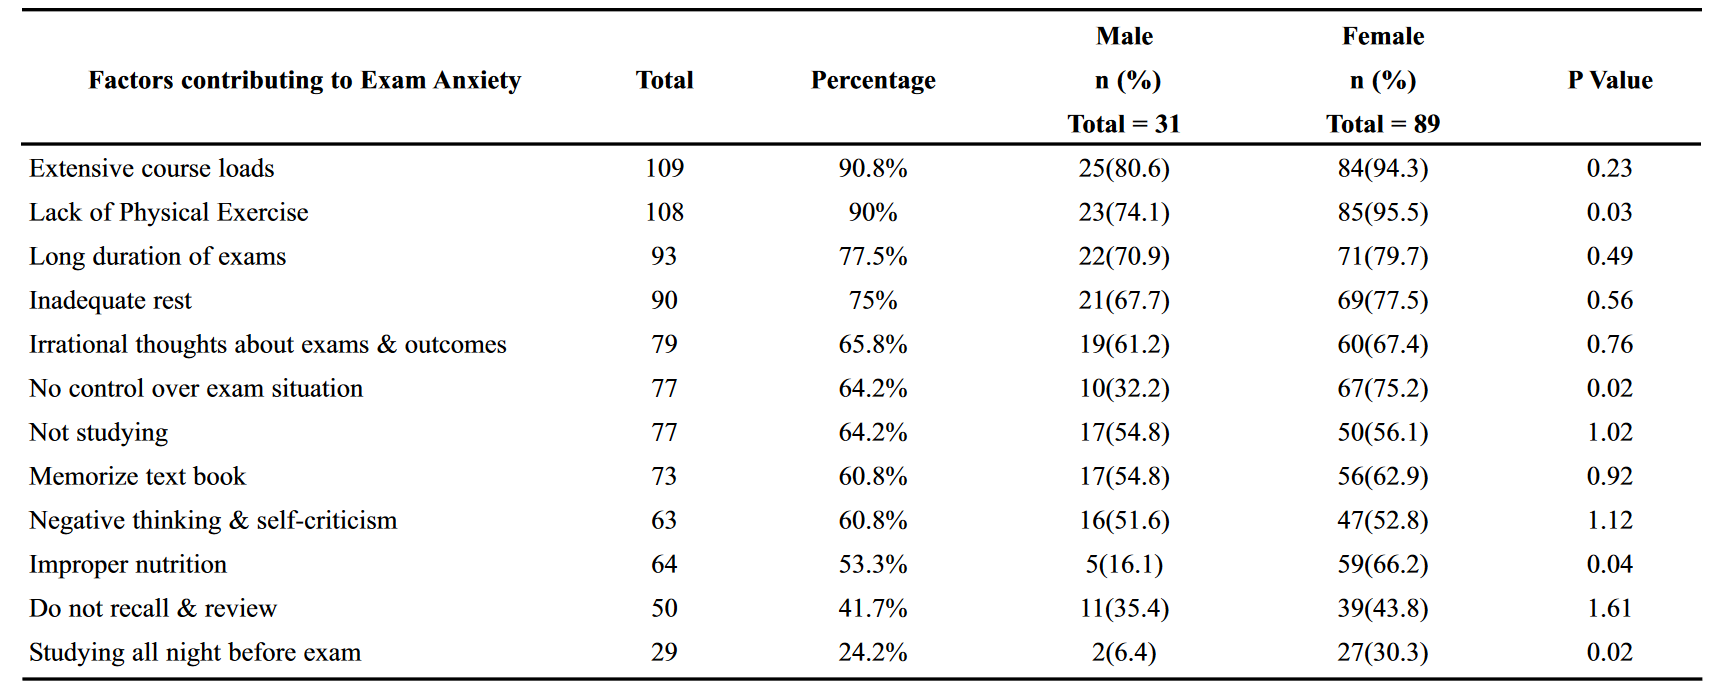
\includegraphics[scale=0.5]{img/jpma_table.png}
		\caption{Ergebnisse der Auswertung (n=120) \cite{hashmat2008factors}}
		\label{fig:jpmatable}
	\end{figure}

	Zum Zusammenhang von Prüfungsangst und exzessiven Kursbelastungen wurde auch \\schon vor 2008 eine Studie durchgeführt, die genau diesen Faktor untersucht. Es wurde auch hier eine positive Korrelation zwischen der Fähigkeit der Studenten Zeit zu managenen, Kursbelastungen aus Sicht der Studenten und Prüfungsangst festgestellt. Hier wurde auf eine ähnliche Art und Weise vorgegangen wie in (Hashmat 2008). \cite{sansgiry2006effect}

	Auch im schulischen Rahmen wird in einer Studie über außerschulisches Leben, Lebensstil und schulbezogenen Ängsten berichtet. Es wird herausgehoben, dass Schulangst / Prüfungs-\\angst im Laufe der Schullaufbahn immer höher wird (und dies vermutlich im Laufe einer tertiären Ausbildung nicht weniger wird) \cite{pixner2013prufungsangst}

	Wie in (Hashmat 2008) berichtet wird, gibt es viele Faktoren, die man beachten kann, um Prüfungsängsten entgegenzuwirken. Zusätzlich dazu ist Selbstwirksamkeitserwartung ein vermutlich großer Faktor auf Prüfungsangst und direkt auch Prüfungsnoten. Es gibt verschiedene intrinsische/extrinsische Quellen dieser Selbstwirksamkeitserwartung die in (Bandura 1977 \cite{bandura1977self}) beschrieben werden.

	Die Ergebnisse der Studie über Selbstwirksamkeitserwartung und Prüfungsangst sind, dass je höher die Prüfungsangst, desto schlechter die daraus resultierende Note. Dennoch konnten die Forscher aufgrund der Ergebnisse nicht klar feststellen, ob Selbstwirksamkeitserwartung direkt zu besseren Prüfungsnoten führt, da kein direkte Korrelation gefunden wurde. \cite{barrows2013anxiety}. Es ist durgehend ersichtlich, dass Prüfungsangst und Prüfungsnoten einen Zusammenhang haben und manchmal die Studenten selbst die Ursachen der Prüfungsangst teilweise behandeln können. Selbstwirksamkeitserwartung spielt auch eine Rolle, wie stark die Prüfungsangst wahrgenommen wird, aber dennoch ist Selbstwirksamkeitserwartung nicht so ein signifikanter Faktor, wie zum Beispiel sportliche Aktivitäten. \cite{barrows2013anxiety} \cite{hashmat2008factors}
\newpage

\bibliography{biblio}{}
\bibliographystyle{alpha}

\end{document}